\section{Wstęp}
\subsection{Cel projektu}
Celem projektu jest wybranie struktury modeli oraz ich identyfikacja na podstawie zebranego zestawu danych. Pierwszy zestaw zawiera pomiary statyki obiektu, drugi natomiast - pomiary jego dynamiki.
\subsection{Wizualizacja danych}
\subsubsection{Dane do modelu statycznego}
Dane potrzebne do wyznaczenia modelu statycznego zostały pobrane z pliku $danestat4.txt$. Zawarte w nim punty zostały przedstawione na wykresie poniżej.
\begin{figure}[H]
\centering
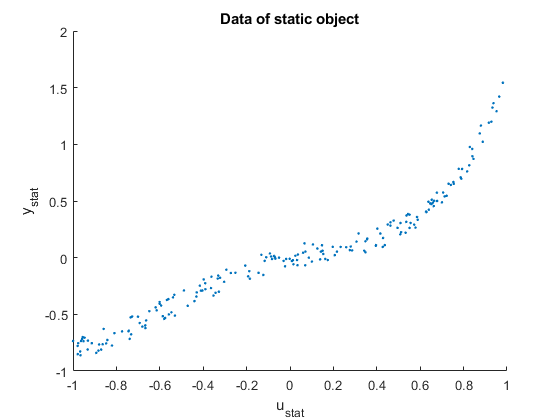
\includegraphics[width=15cm]{images/21.png}
\caption{Zbiór danych wykorzystany do wyznaczenia modelu statycznego.}
\label{fig:1}
\end{figure}
W celu wyznaczenia modelu należało przygotować dane, dzieląc go odpowiednio na zbiór uczący oraz weryfikujący. Przyjęto, że zbiór uczący będzie stanowił 30$\%$ całej bazy danych, natomiast zbiór weryfikujący - pozostałe 70$\%$. Wynik podziału został przedstawiony na wykresie poniżej. Jak widać, zarówno zbiór uczący, jak i weryfikujący, zawierają próbki z prawie całej dziedziny (-1;1).
\begin{figure}[H]
\centering
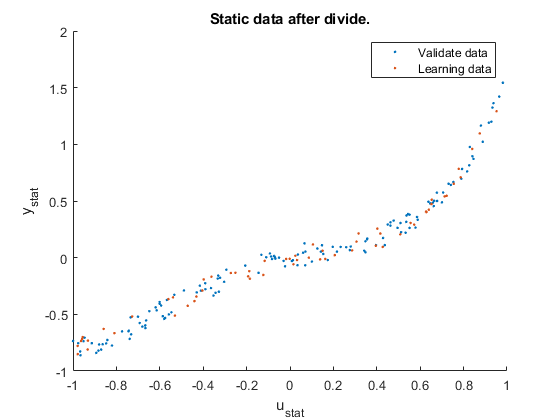
\includegraphics[width=15cm]{images/25.png}
\caption{Zbiór danych wykorzystany do wyznaczenia modelu statycznego po podziale.}
\label{fig:1}
\end{figure}
\subsubsection{Model dynamiczny}
\begin{figure}[H]
\centering
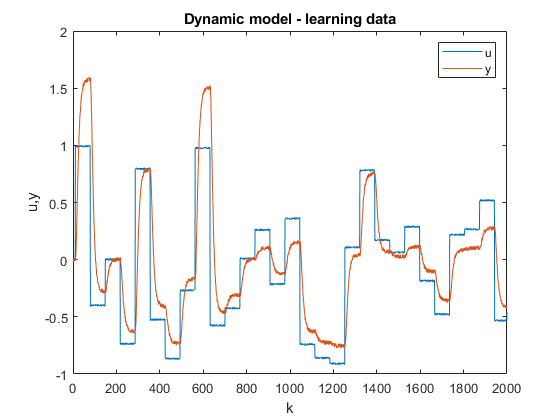
\includegraphics[width=15cm]{images/23.png}
\caption{Dane uczące do modelu dynamicznego.}
\label{fig:2}
\end{figure}
\begin{figure}[H]
\centering
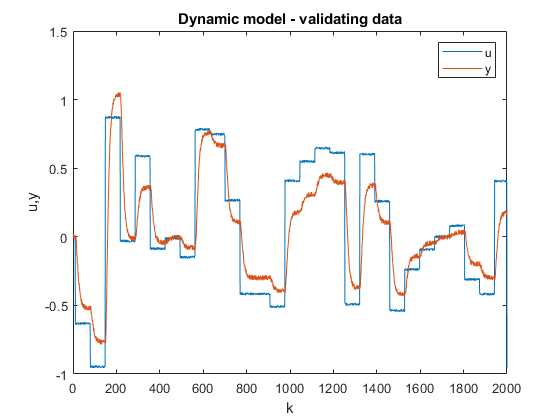
\includegraphics[width=15cm]{images/24.png}
\caption{Dane weryfikujące do modelu dynamicznego.}
\label{fig:3}
\end{figure}
\section{Identyfikacja modeli statycznych}
\subsection{Zestawienie otrzymanych modeli}
\begin{table}[H]
\centering
\begin{tabular}{|c|c|c|c|}
\hline
St. Wielomianu & Współczynniki & $E_{learning}$ & $E_{ver}$ \\ \hline
1              & 0             & 0.016835              & 0.026768         \\ \hline
2              & 0             & 0.013875              & 0.021407         \\ \hline
3              & 0             & 0.005283              & 0.009850         \\ \hline
4              & 0             & 0.002789              & 0.003813         \\ \hline
5              & 0             & 0.002754              & 0.004035         \\ \hline
6              & 0             & 0.002683              & 0.004457         \\ \hline
\end{tabular}
\end{table}
\begin{figure}[H]
\centering
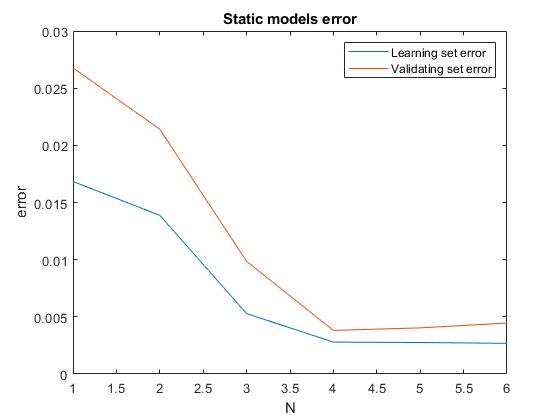
\includegraphics[width=15cm]{images/s_error.png}
\caption{Przebieg wartości błędów modelowania od stopnia modelu.}
\label{fig:s_error}
\end{figure}
\subsection{Wizualna ocena otrzymanych modeli}
\begin{figure}[H]
\centering
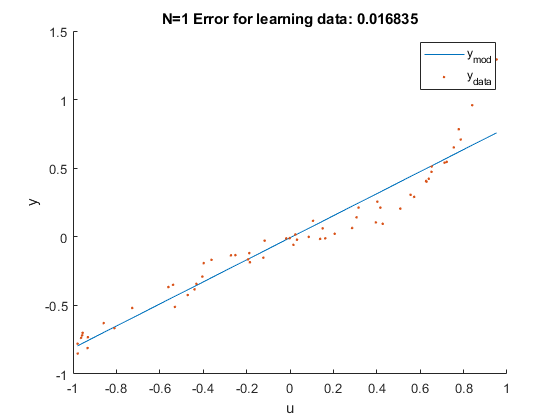
\includegraphics[width=15cm]{images/s1.png}
\caption{Porównanie modelu statycznego 1. rzędu z danymi uczącymi.}
\label{fig:s1}
\end{figure}
\begin{figure}[H]
\centering
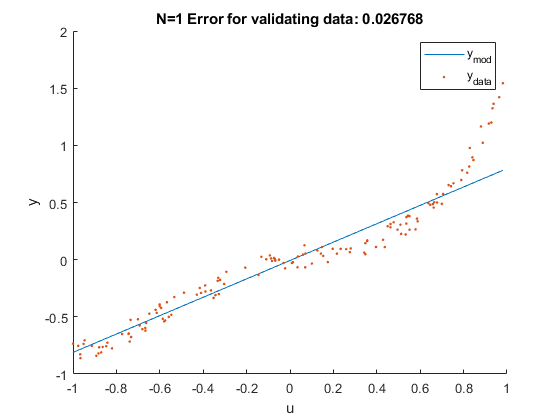
\includegraphics[width=15cm]{images/s2.png}
\caption{Porównanie modelu statycznego 1. rzędu z danymi weryfikującymi.}
\label{fig:s2}
\end{figure}
\begin{figure}[H]
\centering
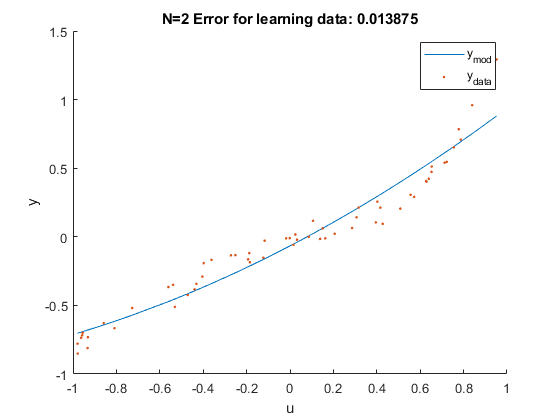
\includegraphics[width=15cm]{images/s3.png}
\caption{Porównanie modelu statycznego 2. rzędu z danymi uczącymi.}
\label{fig:s3}
\end{figure}
\begin{figure}[H]
\centering
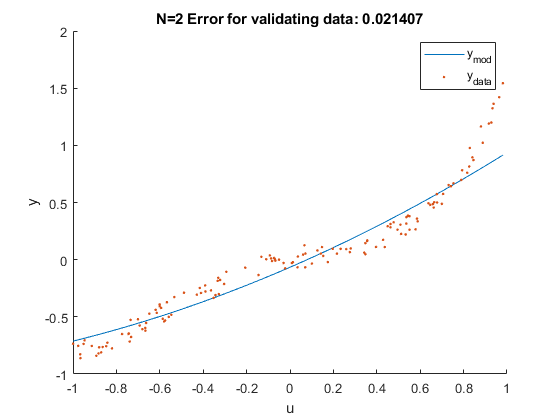
\includegraphics[width=15cm]{images/s4.png}
\caption{Porównanie modelu statycznego 2. rzędu z danymi weryfikującymi.}
\label{fig:s4}
\end{figure}
\begin{figure}[H]
\centering
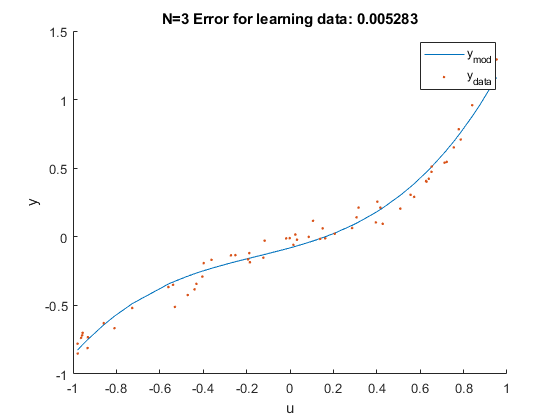
\includegraphics[width=15cm]{images/s5.png}
\caption{Porównanie modelu statycznego 3. rzędu z danymi uczącymi.}
\label{fig:s5}
\end{figure}
\begin{figure}[H]
\centering
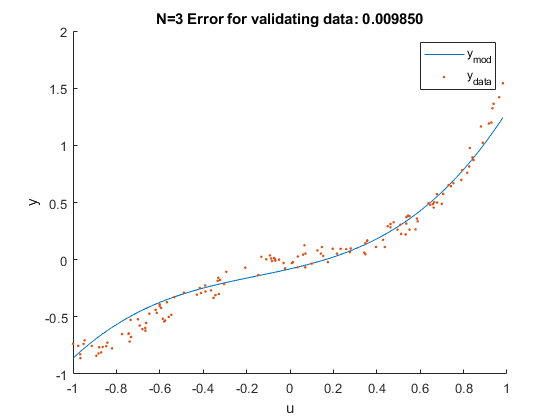
\includegraphics[width=15cm]{images/s6.png}
\caption{Porównanie modelu statycznego 3. rzędu z danymi weryfikującymi.}
\label{fig:s6}
\end{figure}
\begin{figure}[H]
\centering
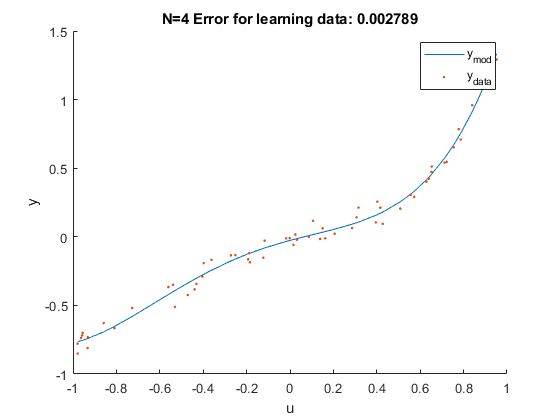
\includegraphics[width=15cm]{images/s7.png}
\caption{Porównanie modelu statycznego 4. rzędu z danymi uczącymi.}
\label{fig:s7}
\end{figure}
\begin{figure}[H]
\centering
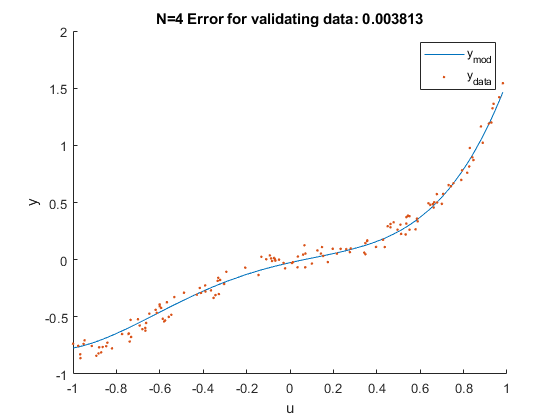
\includegraphics[width=15cm]{images/s8.png}
\caption{Porównanie modelu statycznego 4. rzędu z danymi weryfikującymi.}
\label{fig:s8}
\end{figure}
\begin{figure}[H]
\centering
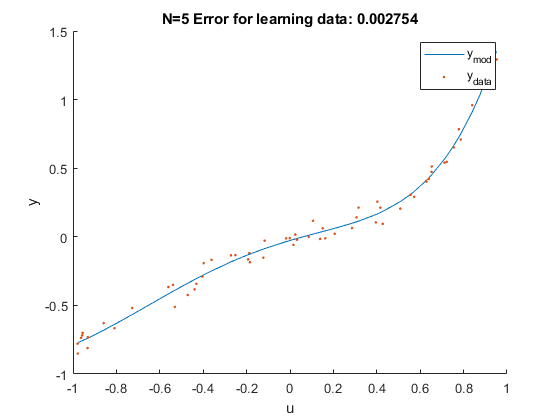
\includegraphics[width=15cm]{images/s9.png}
\caption{Porównanie modelu statycznego 5. rzędu z danymi uczącymi.}
\label{fig:s9}
\end{figure}
\begin{figure}[H]
\centering
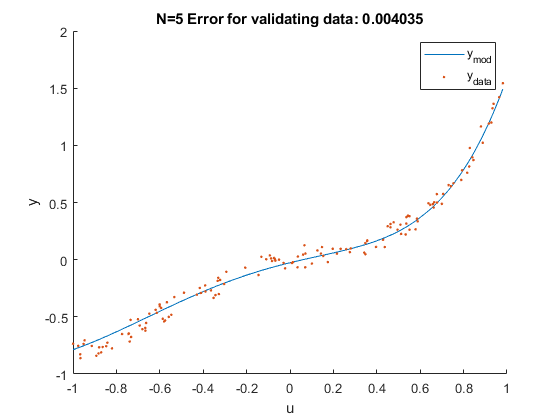
\includegraphics[width=15cm]{images/s10.png}
\caption{Porównanie modelu statycznego 5. rzędu z danymi weryfikującymi.}
\label{fig:s10}
\end{figure}
\begin{figure}[H]
\centering
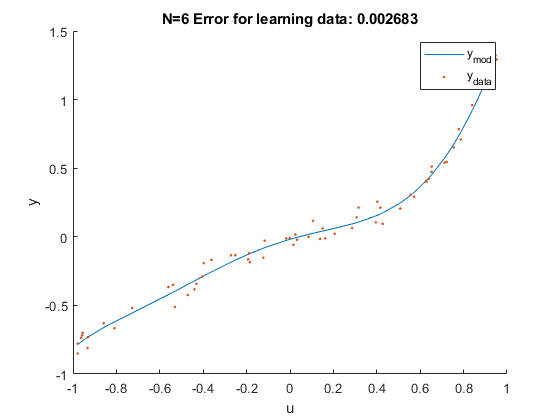
\includegraphics[width=15cm]{images/s11.png}
\caption{Porównanie modelu statycznego 6. rzędu z danymi uczącymi.}
\label{fig:s11}
\end{figure}
\begin{figure}[H]
\centering
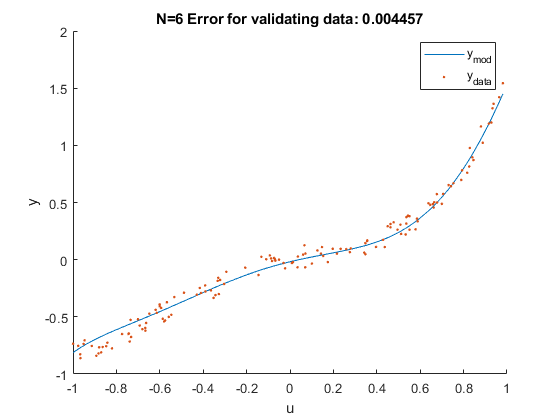
\includegraphics[width=15cm]{images/s12.png}
\caption{Porównanie modelu statycznego 6. rzędu z danymi weryfikującymi.}
\label{fig:s12}
\end{figure}
\subsection{Podsumowanie}
Jako najlepszy model wybrany został model 4. rzędu. Jest to model o najwyższym stopniu, dla którego obserwujemy malejące wartości błędu dla zbioru weryfikującego, to znaczy, że wszystkie modele wyższego stopnia są przewymiarowane, przez co zbytnio dopasowują się do danych zawartych w zbiorze uczącym. Ponadto, pod względem wizualnym, przebiegi modeli powyżej 4. stopnia nie różnią się znacząco między sobą, więc ograniczenie złożoności modelu do 4. stopnia jest wskazane.
\section{Identyfikacja modeli dynamicznych}
\begin{table}[H]
\centering
\begin{tabular}{|c|c|c|c|c|c|c|}
\hline
\multicolumn{3}{|c|}{Rząd modelu}                      & \multicolumn{2}{c|}{ARX}   & \multicolumn{2}{c|}{OE}    \\ \hline
Rząd wielomianu & Rząd dynamiki & Ilość współczynników & $E_{learning}$ & $E_{ver}$ & $E_{learning}$ & $E_{ver}$ \\ \hline
1               & 1             &                      & 0              & 0         & 0              & 0         \\ \hline
1               & 2             &                      & 0              & 0         & 0              & 0         \\ \hline
1               & 3             &                      & 0              & 0         & 0              & 0         \\ \hline
2               & 1             &                      & 0              & 0         & 0              & 0         \\ \hline
2               & 2             &                      & 0              & 0         & 0              & 0         \\ \hline
2               & 3             &                      & 0              & 0         & 0              & 0         \\ \hline
3               & 1             &                      & 0              & 0         & 0              & 0         \\ \hline
3               & 2             &                      & 0              & 0         & 0              & 0         \\ \hline
3               & 3             &                      & 0              & 0         & 0              & 0         \\ \hline
4               & 1             &                      & 0              & 0         & 0              & 0         \\ \hline
4               & 2             &                      & 0              & 0         & 0              & 0         \\ \hline
4               & 3             &                      & 0              & 0         & 0              & 0         \\ \hline
\end{tabular}
\end{table}
\section{Charakterystyka statyczna na podstawie modelu dynamicznego}